% !TEX TS-program = pdflatex
% !TEX encoding = UTF-8 Unicode

\documentclass[presentation,svgnames,12pt]{beamer}

%\usepackage{pgfpages} %for {show notes on second screen option}

\mode<presentation>
{
  %\usetheme{Rochester} %pretty plain, no footer and progress
  %\usetheme{Marburg}   %sidebar with all (sub)sections
  %\usetheme{Madrid}	%footer with author, title, date and frame number, 
  %\usetheme{Luebeck}		%big header with all sections, footer with author and title
  \usetheme{Frankfurt}  %favorite for now %header with progress
  %\usetheme{Dresden}	%header with progress, 2 footers for author an title
  %\usetheme{Copenhagen}	%big header with all sections, footer with author and title
  %\usetheme{Berlin}		%header with progress, 2 footers for author an title
  %\usetheme{Warsaw}		%big header with all sections, footer with author and title

%\setbeamercolor*{palette primary}{use=structure,fg=white,bg=FireBrick}
%\setbeamercolor{item}{fg=FireBrick}
%\setbeamercolor{section in toc}{fg=FireBrick}
\useinnertheme{circles} %bullet points look nice to me that way (especially numbered ones)
%\usecolortheme{crane}

\setbeamertemplate{footline}
{
  \leavevmode%
  \hbox{%
  \begin{beamercolorbox}[wd=.45\paperwidth,ht=2.25ex,dp=1ex,center]{author in head/foot}%
    \usebeamerfont{author in head/foot}\insertshortauthor
  \end{beamercolorbox}%
  \begin{beamercolorbox}[wd=.45\paperwidth,ht=2.25ex,dp=1ex,center]{title in head/foot}%
    \usebeamerfont{title in head/foot}\insertshorttitle\hspace*{3em}
  \end{beamercolorbox}%
  \begin{beamercolorbox}[wd=.1\paperwidth,ht=2.25ex,dp=1ex,center]{author in head/foot}%
    \insertframenumber{} / \inserttotalframenumber\hspace*{1ex}  
  \end{beamercolorbox}}%

  \vskip0pt%
}

  %\setbeamercovered{transparent}
  % or whatever (possibly just delete it)

\setbeamertemplate{navigation symbols}{}%remove navigation symbols
%\setbeameroption{show notes on second screen}
}

\usepackage[ngerman]{babel}
\usepackage[utf8x]{inputenc}
\usepackage[T1]{fontenc}
\usepackage{eurosym} %for euro symbol via \euro

\usepackage{lmodern}

%stuff used for the tables
\usepackage{tabularx}
\usepackage{hhline}

\definecolor{XBoneGreen}{RGB}{16, 124, 16}
\definecolor{XBoneLightGreen}{RGB}{93, 194, 30}

\title[OpenLDAP- und FreeRADIUS-Server]   % (optional, use only with long paper titles)
{Aufsetzen eines OpenLDAP- und FreeRADIUS-Servers}

\subtitle
{Abschlusspräsentation des Projektes im Rahmen der Ausbildung zum Fachinformatiker Systemintegration} % (optional)

\author % (optional, use only with lots of authors)
{Sebastian Deußer}
%\date{13. Juli 2015}
%\logo{
\includegraphics[scale=0.05]{Bilder/logo_ti.png}}

\subject{Aufsetzen eines OpenLDAP- und FreeRADIUS-Servers}
% This is only inserted into the PDF information catalog. Can be left
% out. 

% If you have a file called "university-logo-filename.xxx", where xxx
% is a graphic format that can be processed by latex or pdflatex,
% resp., then you can add a logo as follows:

% \pgfdeclareimage[height=0.5cm]{university-logo}{university-logo-filename}
% \logo{\pgfuseimage{university-logo}}

% If you wish to uncover everything in a step-wise fashion, uncomment
% the following command: 
%\beamerdefaultoverlayspecification{<+->}

\institute[ti]{taylorix institut für berufliche Bildung e.V.}
\keywords{LDAP, RADIUS, LaTeX, Graphviz}

\begin{document}
\setcounter{framenumber}{-1}
{
\setbeamertemplate{footline}{}
\frame{\titlepage}
}

\section{}
\begin{frame}{Übersicht}
\tableofcontents
\end{frame}
\note{}

\let\olditemize\itemize %bullets should have more space between them
\renewcommand\itemize{\olditemize\addtolength{\itemsep}{12pt}}

\let\oldenumerate\enumerate %enums too
\renewcommand\enumerate{\oldenumerate\addtolength{\itemsep}{12pt}}


\section{Projektbeschreibung}
\subsection{}
\begin{frame}{Projektumfeld: Firmenbeschreibung fgn GmbH}
\begin{columns}[c]
	\begin{column}{2.5cm}
		
\includegraphics[scale=0.7]{Bilder/logo_fgn.png}
	\end{column}
\end{columns}
\vspace{8pt}
\begin{itemize}
	\item fgn GmbH gegründet 1996 als TU Spin-Off
	\item Kerngeschäft Netzwerkschulungen und -consulting
	\item circa ein Dutzend Mitarbeiter
	\item eigene Server und Schulungslabore im DFKI Neubau
\end{itemize}
\end{frame}


\begin{frame}{Ausgangssituation}
\begin{itemize}
	\item CommuniGate-Server für E-Mail und Identity Management
	\item Identity Management genutzt für die meisten Logins
	\item E-Mail-Server verwaltet drei E-Mail-Domains
	\item Internetanbindung über TU Kaiserslautern
\end{itemize}
\end{frame}


\section{Planung}
\subsection{}
\begin{frame}{Anforderungen Ersatzserver}
\begin{itemize}
	\item LDAP-Server
	\item RADIUS-Server
	\item Anwenderkonten übernehmen
	\item Absichern per Firewall
\end{itemize}
\end{frame}

\begin{frame}{Konzept Ersatzserver}
\begin{itemize}
	\item ESXi-VM mit Linux (Debian 8.0)
	\item OpenLDAP-Server
	\item FreeRADIUS-Server
	\item FreeRADIUS-Server an OpenLDAP-Server anbinden
	\item Anwenderkonten per Skript importieren
\end{itemize}
\end{frame}


\section{Realisierung}
\subsection{Realisierung des Ersatzservers}
\begin{frame}{Realisierung des Ersatzservers (1)}
\begin{itemize}
	\item LDAP-over-SSL als einzige externe Zugriffsmöglichkeit
	\item endgültige Verzeichnisstruktur:
\end{itemize}
\centering
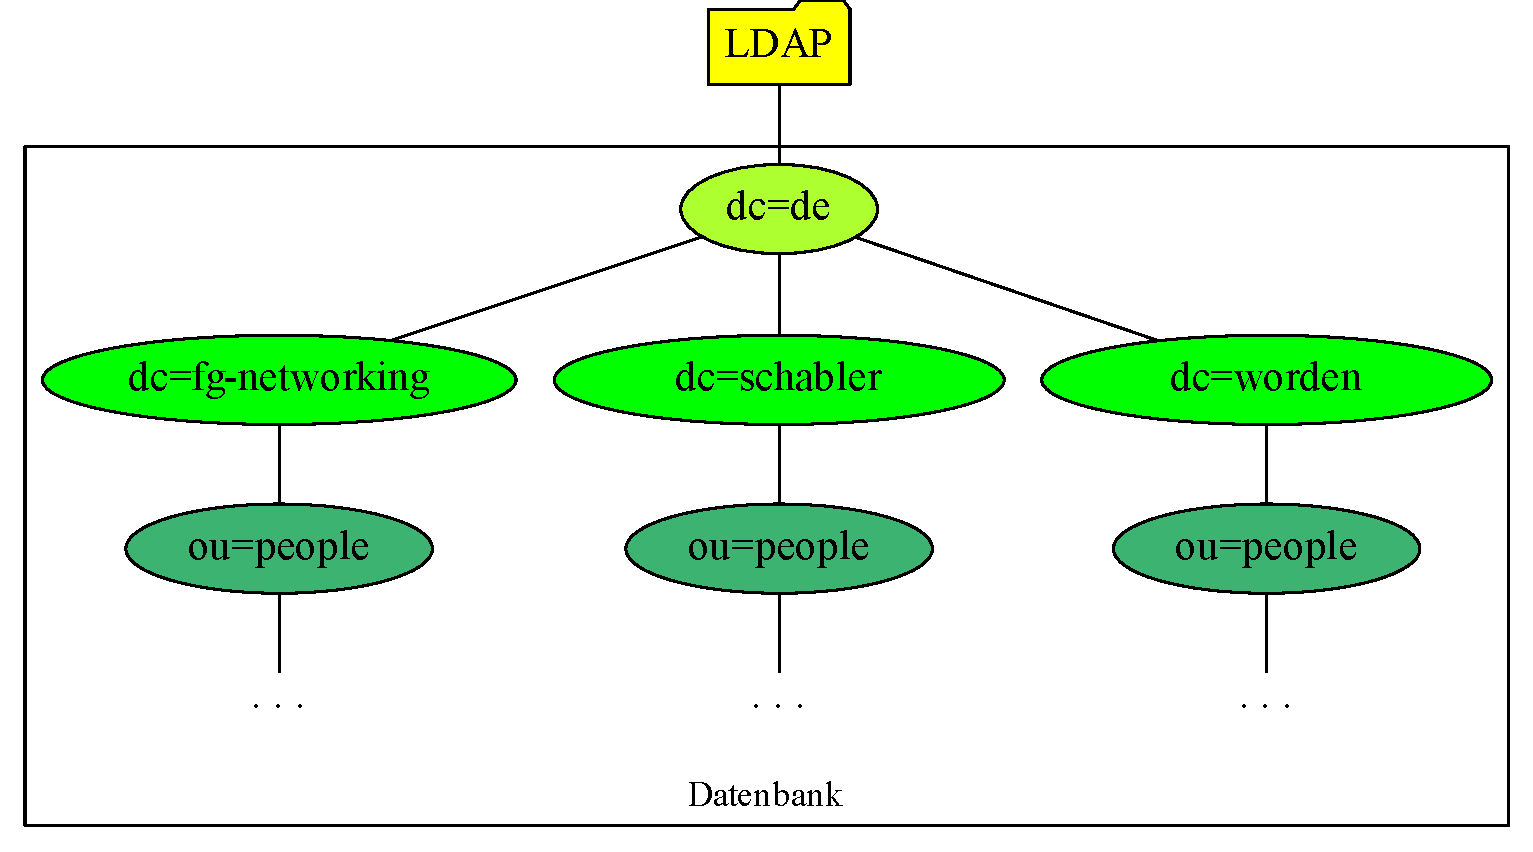
\includegraphics[width=\textwidth]{Bilder/LDAP-fgn.pdf}
\end{frame}


\begin{frame}{Realisierung des Ersatzservers (2)}
\begin{itemize}
	\item Shared Secret für TU E-Mail-Server konfiguriert
	\item Anbindung an LDAP über mitgeliefertes Modul
	\item Anbindung der Webservices und OpenVPN
	\item Import von Anwenderkonten per generierter LDIF-Datei
\end{itemize}
\end{frame}


\section{Qualitätssicherung}
\subsection{Qualitätssicherung}
\begin{frame}{Qualitätssicherung}
\begin{enumerate}
	\item Funktionstests:
	\vspace{6pt}
	\begin{itemize}
		\item Login bei Webservices und OpenVPN nach Umstellung getestet
		\item FreeRADIUS Test mit \texttt{radtest}
	\end{itemize}
	\item Sicherheitstests:
	\vspace{6pt}
	\begin{itemize}
		\item Anmelden mit falschen Anmeldeinformationen
		\item Überprüfung OpenSSH-Server Konfiguration
		\item Port-Scan mit \texttt{nmap} (aus fgn-Netz und extern)
	\end{itemize}
\end{enumerate}
\end{frame}

\subsection{Probleme und Lösungen}
\begin{frame}{Probleme und Lösungen}
\begin{enumerate}
	\item Design der LDAP-Baumstruktur
	\vspace{6pt}
	\begin{itemize}
		\item ursprüngliche Idee eine Datenbank pro Domain
	\end{itemize}
\end{enumerate}
\vspace{6pt}
\centering
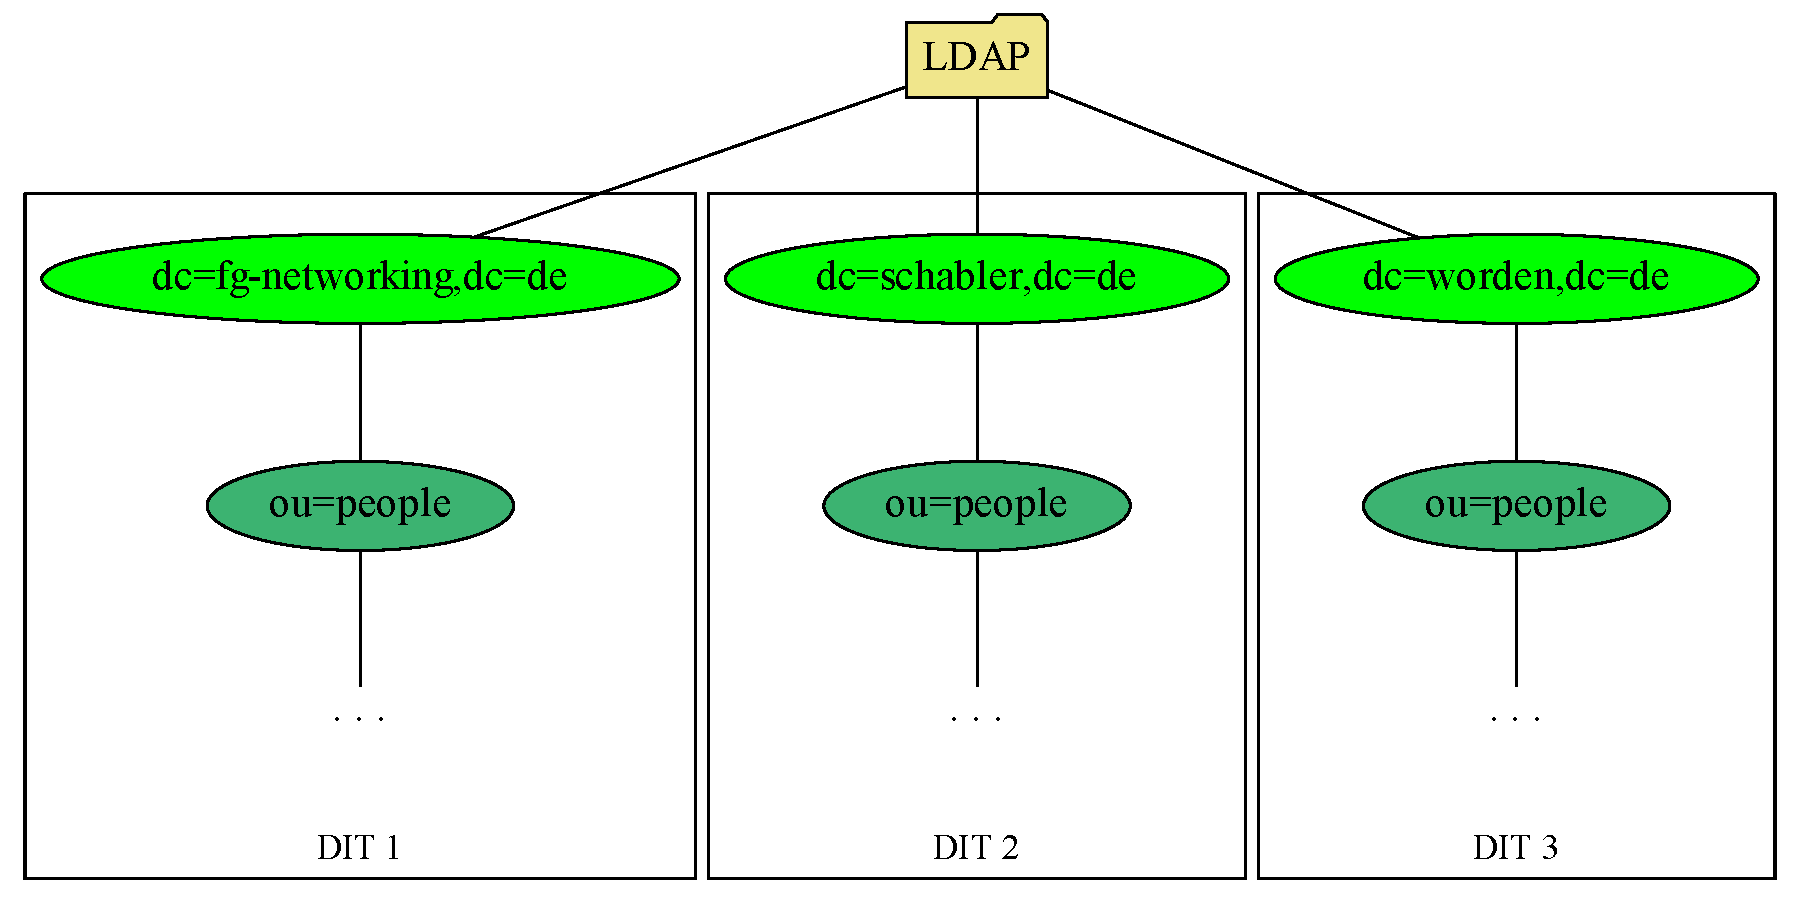
\includegraphics[width=\textwidth]{Bilder/LDAP-fgn-planned.pdf}
\end{frame}

\begin{frame}{Probleme und Lösungen (2)}
\begin{enumerate}
	\setcounter{enumi}{1}
	\item Egroupware
	\vspace{6pt}
	\begin{itemize}
		\item fehlendes Passwort für Installer
		\item Zuständiger in Urlaub
	\end{itemize}
	\medskip
	\item RADIUS Praxistests nicht möglich
	\vspace{6pt}
	\begin{itemize}
		\item FreeRADIUS mit \texttt{radtest} getestet
		\item bei E-Mail-Server Anbindung nachholen
	\end{itemize}
\end{enumerate}
\end{frame}

\section{Projektabschluss}
\subsection{Projektkosten}
\begin{frame}{Projektkosten (mit Vergleich zu Alternative)}
\begin{table}
\centering
	\begin{tabularx}{0.9\textwidth}{|X|r|r|}
		\hline
		 	&	OpenLDAP \& &	CommuniGate-\\
		Kosten-Kategorie	&	FreeRADIUS &	Upgrade\\
		\hline
		Hardware &	0,00\euro{} &	0,00\euro{}\\
		\hline
		Softwarelizenzen &	0,00\euro{} &	1.849,00\euro{}\\
		\hline
		Arbeitsaufwand &	2.485,00\euro{} &	2.485,00\euro{}\\
		\hhline{|=|=|=|}
		Gesamt &	2.485,00\euro{} &	4.334,00\euro{}\\
		\hline
	\end{tabularx}
\end{table}
\bigskip
Amortisation nach knapp 15 Monaten gegenüber weiterer Nutzung des alten CommuniGate-Servers
\end{frame}

\subsection{Fazit}
\begin{frame}{Fazit}
\begin{itemize}
	\item alle Systeme außer Egroupware, E-Mail-Server umgestellt
	\item FreeRADIUS noch kein Praxistest
	\item Zeitplanung nicht optimal:
	\vspace{6pt}
	\begin{itemize}
		\item[--] zu wenig Zeit für Design der Verzeichnisstruktur veranschlagt
		\item[--] für Vorbereitungen mehr Zeit eingeplant als benötigt
	\end{itemize}
\end{itemize}
\end{frame}


\subsection{Ausblick}
\begin{frame}{Ausblick}
Erweiterungsmöglichkeiten:
\vspace{6pt}
	\begin{itemize}
		\item Anbindung neuer E-Mail-Server
		\item Ersatz lokaler Accounts
		\item Anbindung Managed Switches an FreeRADIUS
		\item Samba-Domäne für Windows Rechner
	\end{itemize}
\end{frame}


\section{} %section shall not be visible in navbar, hence empty name
\begin{frame}{Fin}
	\bigskip\bigskip\bigskip\bigskip\bigskip\bigskip
	Vielen Dank für Ihre Aufmerksamkeit
	
	Für Fragen stehen ich ihnen selbstverständlich zur Verfügung
	
	\bigskip\bigskip\bigskip
	\bigskip
	\bigskip
	\bigskip Diese Präsentation wurde mit \LaTeX{}-Beamer erstellt
	
	Grafiken erstellt mit GraphViz
\end{frame}


%\subsection{Projektkosten - Wartung}
%\begin{frame}{Projektkosten - Wartung}
%	\begin{tabularx}{\textwidth}{|X|r|r|r|}
%%		\hline
%%		\mcc{4}{Jährliche Kosten}\\
%		\hline
%		Kosten-	&	OpenLDAP \& &	CommuniGate- &	\\
%		Kategorie	&	FreeRADIUS &	Upgrade &	Status Quo\\
%		\hline
%		Hardware &	0,00\euro{} &	0,00\euro{} &	0,00\euro{}\\
%		\hline
%		Softwarelizenzen &	0,00\euro{} &	332,82\euro{} &	0,00\euro{}\\
%		\hline
%		Arbeitsaufwand &	355,00\euro{} &	213,00\euro{} &	2.350,00\euro{}\\
%		\hhline{|=|=|=|=|}
%		Gesamt &	355,00\euro{} &	545,82\euro{} &	2.350,00\euro{}\\
%		\hline
%	\end{tabularx}
%\end{frame}

\end{document}